\newpage
\subsection{Scrum}

\label{sec:scrumProjectManagement}

The Scrum approach is an iterative and incremental agile software development
framework that consists of three phases: The outline planning phase, which is
followed by a series of sprint cycles, and lastly a project closure phase. This process is illustrated in figure~\ref{fig:scrumProcess}.

The product owner adds user stories to the product backlog. A user story is a short sentence that describe a small piece of functionality the user wants in the system. The user stories are selected from the product backlog and moved to the sprint backlog at the beginning of a sprint. This process is repeated until the limit of available work hours is reached. 

The user stories in the sprint backlog are then broken down into tasks and assigned. Each sprint has a duration of one to four weeks and has three important parts: The first part is the
planning meeting, then the daily  meetings, and finally, the process is
concluded with an end meeting. 
\begin{figure}[H]
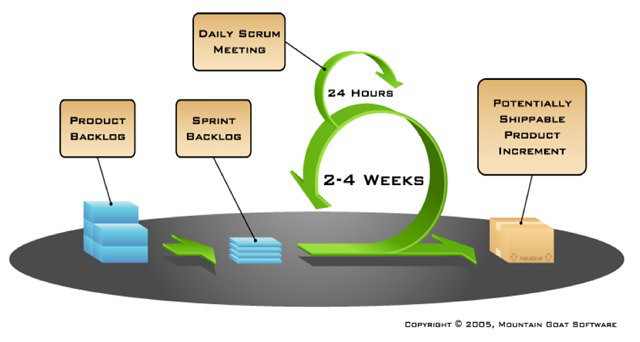
\includegraphics[width=\textwidth]{ch/projectManagement/fig/sprintProcess.jpg}
\caption{Illustration of the process in Scrum}
\label{fig:scrumProcess}
\end{figure}


\subsubsection{Sprint planning}
\label{sec:sprintplanning}
The objective of sprint planning is to find out what work that needs to be completed within the duration of the sprint. This is done by preparing a sprint backlog that consists of tasks, namely the user stories. The estimation of each user story is based on how much time the team think it will take to complete, on previous experiences, or lack of it, and difficulty level. In the Scrum approach, planning poker is a common strategy to use for time planning~\cite{planningpoker}.

\subsubsection{Planning poker}
In planning poker, each team member individually decide on how many units of time they think a task and/or user story will require to complete. This is repeated for each task and/or user story. The units of time can be in hours, work days, or whatever unit the team sees fit.

When a user story is presented, every team member presents the unit they believe the user story will require. If the entire team agrees on one estimate per user story, the user story is assigned that particular estimate. If not, the team members must defend their choices and come to a conclusion the entire team agrees upon.

\subsubsection{Daily meetings}
A work day is usually initiated with a daily meeting. The purpose of these meetings is to give an overview to the entire team of what all the other members are working on. For about fifteen minutes, all the team members briefly summarize which tasks they have performed and whether something went wrong.

By having this meeting, the team would quickly become aware if something was interrupting the development process. This can be a poorly estimated user story that requires more thought and replanning, or some other risk that may occur. For a full list of risks and their remedial actions, see section~\ref{sec:risk}. 

\subsubsection{End meeting}
The end meeting is held at the end of each sprint. This meeting consists of a sprint review and a retrospective discussion of the previous sprint. The purpose of this is to ensure that the project is progressing as planned. It is typical to have meetings with the customer at the end of each sprint to review the product. This gives the customer the opportunity to provide feedback on the product and affect the direction the development.


